
\chapter{Implementierung}
\label{chapter-implementierung}
Das folgende Kapitel beschreibt die Implementierung des Backends,
Reservierungsinterfaces sowie des Fontends. Zunächst wird die Implementierung
des Reservierungsinterfaces und die damit einhergehende technischen Aspekten
beschreiben. Bei wird aufschluss über die Struktur gegben und die
Kernfunktionalität sowie Sackgassen in der Realisierung werden näher erläutert.
Daraufhin wird die Umsetzung des Frontend beschreiben. Abschließend wird auf die
Inbetriebnahme des Systems eingegangen.


\section{Implementierung des Reservierungsinterfaces}
Der Abschnitt beschreibt die Struktur des Reservierungsinterface mit seinen
technischen Aspekten und die Implementierung der Funktionalitäten
(\ref{section:funktionale}). Zunächst wird die Implementierung der
Kernfunktionalitäten erläutert. Daraufhin werden Sackgassen thematisiert.


\subsection{Struktur des Reservierungsinterface}
Das folgende Unterkapitel geht auf die Strukturen und Teilkomponenten des
Reservierungsinterface ein. In \ref{fig:db} wird die Verzeichnisstruktur
präsentiert. Das Reservierungsinterface teilt sich in drei wesentliche
Bausteine: \textit{node, SQLit(prisma)} und \textit{server.ts} .

\begin{figure}[h]
  \centering
  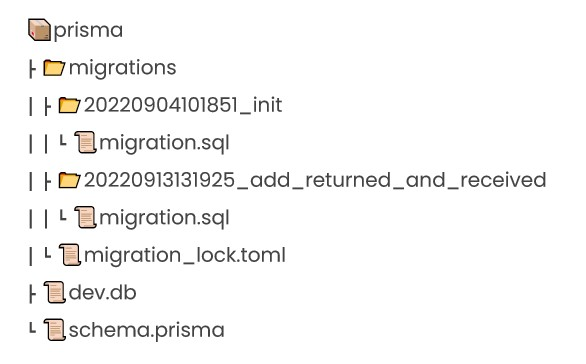
\includegraphics[scale=0.7]{Bilder/Db.jpg}
  \caption[Verzeichnisstruktur des Reservierungsinterfaces]{Verzeichnisstruktur des Reservierungsinterfaces}
  \label{fig:db}
\end{figure}

Der \textit{node} Ordner gibt... .

\textit{prisma} macht Dinge

\textit{server.ts} für Routen

\subsection{Implementierung der Kernfunktionalität}
Dieser Abschnitt präsentiert die Implementierung der Kernfunktionalität des
Zwischenbackends, welche aus den Anforderungen  bestimmt wurden
(\ref{section:anforderung}). Bei der Funktionalität handelt es sich um das
Reservieren in die Zukunft, sowie das Speichern dieser Vorgänge und die damit
einhergehende Bestätigung für die Aktualisierung in Snipe-IT.

Um auf die Assets zugreifen zu können wurde mit der Snipe-IT JSON REST API
gearbeitet. Die api HIER AUFBAU ERKLÄREN.

Um mit der api arbeiten zu können muss ein \textit{API
  key}\footnote{\url{https://snipe-it.readme.io/reference/generating-api-tokens}}
  generiert werden. Da persönliche Zugriffstoken verwendet werden, spiegeln die
  Berechtigungen des API-Tokens die Berechtigungen des Nutzenden wider. Das
  bedeutet auch, das die Token lediglich manuell im Dashboard generierbar sind.
  Was zur folge hat, dass das geplante LDAP-System der Universität zu Lübeck
  nicht ohne umstände eingebunden und entsprechend genutzt werden kann. Snipe-IT
  gibt unter anderem die Möglihkeit, das LDAP
  Formular\footnote{\url{https://snipe-it.readme.io/docs/ldap-sync-login}}
  einfach einzubinden, trotzdessen besteht das Problem, der Autentifizierung
  sowie generierung der Tokens offen, da die Daten im Reservierungsinterface bis
  dato nicht übertragen wurdne.


FÜR FRONTEND benötigte Ressourcen: Routen angelegt -> Fastify genutzt, für
vereinfachung


Reservierung in der Zukunft: Daten zwischenspeichern, weil Snipe IT doof ->
SQLite -> Prisma (für einfache verwaltung -> Beispeil und wie es Funktioniert)


Statuseingabe/Ausleihen schwer und komisch -> rumarbeiten

\section{Implementierung des Frontends}
\begin{itemize}
  \item v-calender für den Kalender -> Kalender als wichtiger bestandteil ->
        viel ausbaumöglichkeiten
  \item Tailwindcss für das Styling
  \item Preline für UI -> Nicht empfehlenswert (Sackgassen)
  \item Headless ui für animation
  \item Basiskomponenten, für sich wiederholende und oft eingesetzte elemente
  \item Aufteilung mit dem Bindestrich: Kategorien im Frontend
\end{itemize}



Bei der Implementierung wurde sich an den best practices der
Vue.js-Dokumentation orientiert \todo{(Vue.js, 2021a)}. Zunächst wurde für die
in \ref{subsection:system} Components eine eigene View erstellt.


\section{Nutzung des Systems}
Um das System Nutzen und weiterentwicklen zu können muss... API KEy generieren
lassen

\section{Fazit der Implementierung}